\documentclass[svgnames,compress,12pt,aspectratio=169]{beamer}

\usetheme{Arguelles}

\usepackage{graphics}
\usepackage{minted}
\usepackage{tikz-timing}
\usepackage{tikz}
\usepackage{circuitikz}
\usetikzlibrary{arrows,arrows.meta,shapes,snakes,automata,backgrounds,petri,%
  decorations.pathreplacing,calligraphy,patterns,%
  patterns.meta,pgfplots.groupplots,positioning,shapes.geometric,%
  fit,tikzmark,overlay-beamer-styles,shadows,intersections}
\usepackage{xcolor}

%\beamertemplatenavigationsymbolsempty
%\setbeamertemplate{footline}[frame number]
\setbeamerfont{alerted text}{series=\bfseries}

\newcommand\rtlblock{\textsc{RtlBlock}}
\newcommand\rtlpar{\textsc{RtlPar}}
\newcommand\rtlpath{\textsc{RtlPath}}
\newcommand\rtl{\textsc{Rtl}}
\newcommand\mrtl[1]{\hbox{\mrtlinline|#1|}}
\newcommand\htl{\textsc{Htl}}
\newcommand\abstr{\textsc{Abstr}}
\newcommand\constr{\textsc{Constr}}
\newcommand\ltl{\textsc{Ltl}}

\tikzset{
blacknum/.style={
  circle, draw=none,
  fill=black, inner sep=0pt,
  outer sep=0pt, minimum size=0.9em, text=white, font=\scriptsize\sf\bfseries}
}

\newcommand\blacknum[1]{%
\begin{tikzpicture}[baseline=-0.3em]%
\node[blacknum](a){#1};%
\end{tikzpicture}%
}

\tikzset{
diagonal fill/.style 2 args={fill=#2, path picture={
\fill[#1] (path picture bounding box.south west) -|
                         (path picture bounding box.north east) -- cycle;}}
}

\begin{document}

\title{Formal Verification of High-Level Synthesis}
\subtitle{Thesis Overview}
\author{Yann Herklotz}
\institute{Imperial College London}
\event{PhD Viva}
\date{\small Supervised by John Wickerson \\[1em] 19$^{\mathsf{th}}$ of April, 2024}
%\date{19$^{\mathsf{th}}$ of April, 2024}

\maketitle

\begin{frame}
  \frametitle{Motivation}

  \begin{columns}
    \begin{column}{0.5\linewidth}
      \begin{itemize}
      \item Functional properties of hardware are easier to express at a higher
        level.
      \item Avoid testing these properties again at the hardware level.
      \item Assumes a \alert{reliable} high-level synthesis tool.
      \end{itemize}
    \end{column}
    \begin{column}{0.5\linewidth}
      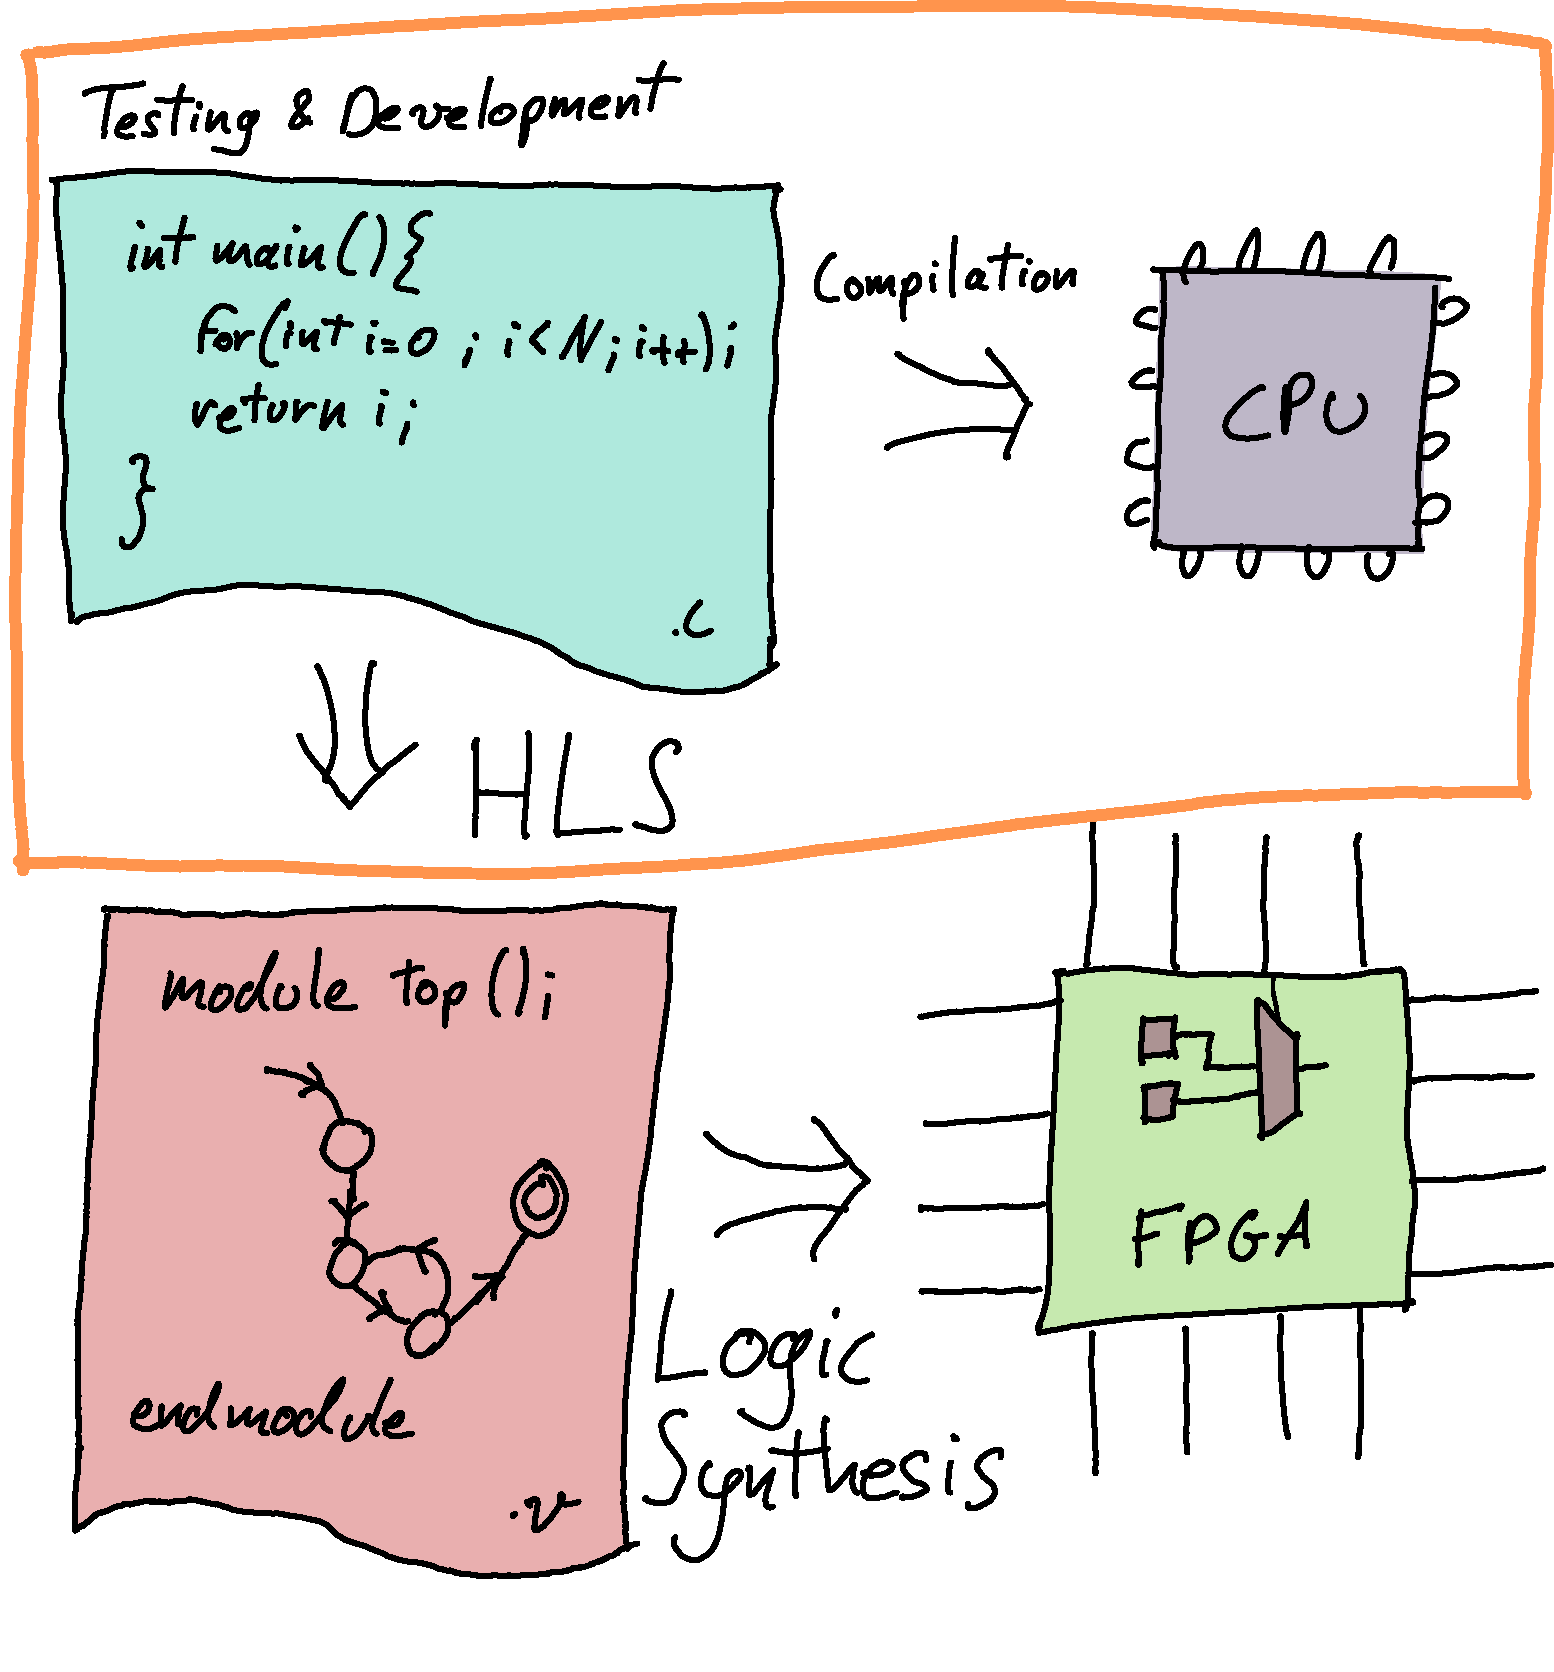
\includegraphics[width=6cm]{hls-flow-testing}
    \end{column}
  \end{columns}
\end{frame}

\begin{frame}
  \frametitle{Thesis overview}

  \begin{block}{Chapter 3}
    Describes the overall structure and design decisions made in Vericert.
  \end{block}

  \begin{block}{Chapter 4}
    Describes the overall correctness theorem and target hardware semantics.
  \end{block}

  \begin{block}{Chapter 5}
    Verify hyperblock scheduling, a critical optimisation in high-level synthesis.
  \end{block}

  \begin{block}{Chapter 6}
    Describe the translation from software into hardware through multiple passes.
  \end{block}
\end{frame}

\begin{frame}
  \frametitle{Chapter 3 \& 4: Design of Vericert and its correctness theorem}

\definecolor{bgbox1}{HTML}{b3e2cd}
\definecolor{bgbox2}{HTML}{cbd5e8}
\definecolor{bgbox3}{HTML}{fdcdac}
\definecolor{ircolor}{HTML}{e78ac3}

\tikzset{
  numlabel/.style={draw,circle,inner sep=0.5mm,fill=white},
  ir/.style={draw,very thick,black, fill=ircolor!70, align=center},
  pass/.style={draw, very thick, rounded corners, fill=white, align=center},
  extpass/.style={draw, dotted, very thick, rounded corners, fill=white, align=center},
  bgbox/.style={draw=none},
  ed/.style={->, very thick, >=stealth},
}

\begin{tikzpicture}[
yscale=-1,
font=\small,
]
\node[ir] (clight) at (0,0) {\strut Clight};
\node[pass] (ccfront) at (2,0) {CompCert \\ frontend};
\node[ir] (rtl) at (4,0) {\strut \rtl};
\node[pass] (dataflow) at (6,0) {dataflow \\ optimisations};
\node[ir] (ltl) at (8,0) {\strut \ltl};
\node[pass] (ccback) at (10,0) {CompCert \\ backend};
\node[ir] (asm) at (12,0) {\strut \textsc{Asm}};

\node[pass] (fsm) at (6,2) {FSM \\ generation};
\node[ir] (htl) at (8,2) {\strut \htl};
\node[pass] (vback) at (10,2) {Vericert \\ backend};
\node[ir] (verilog) at (12,2) {\strut Verilog};

\node[pass] (bbs) at (3.1,2) {\strut find BBs};
\node[ir] (rtlb) at (3.1,4) {\strut \rtlblock};
\node[pass] (ifc) at (0.7,4) {\strut if-conversion};
\node[pass] (sched) at (5.3,4) {\strut schedule};
\node[ir] (rtlp) at (7.3,4) {\strut \rtlpar};
\node[pass] (fsub) at (10.2,4) {\strut forward  substitution};

\node[anchor=north east, align=right] (cclabel) at (12.8,-1.1)
{\textbf{CompCert}};
\begin{pgfonlayer}{background}
\draw[bgbox, fill=bgbox1] (-0.8,-1.1) rectangle (12.8, 0.7);
\end{pgfonlayer}

\node[anchor=north east, align=right] (vlabel) at (12.8,0.9) {\textbf{OOPSLA 2021}};
\begin{pgfonlayer}{background}
\draw[bgbox, fill=bgbox2] (4.5,0.9) rectangle (12.8, 2.7);
\end{pgfonlayer}

\node[anchor=north east, align=right] (thislabel) at (12.8,2.9) {\textbf{PLDI 2024}};
\begin{pgfonlayer}{background}
\draw[bgbox, fill=bgbox3] (-0.8,0.9) -- (4.3,0.9) -- (4.3,2.9) -- (12.8,2.9) --(12.8,4.7) -- (-0.8,4.7) -- cycle;
\end{pgfonlayer}

\draw[ed] (clight) to (ccfront);
\draw[ed] (ccfront) to (rtl);
\draw[ed] (rtl) to (dataflow);
\draw[ed] (dataflow) to (ltl);
\draw[ed] (ltl) to (ccback);
\draw[ed] (ccback) to (asm);
\draw[ed] (rtl) to (fsm);
\draw[ed] (fsm) to (htl);
\draw[ed] (htl) to (vback);
\draw[ed] (vback) to (verilog);
\draw[ed] (rtl) to (bbs);
\draw[ed] (bbs) to (rtlb);
\draw[ed] (rtlb) to[bend left=5] (ifc);
\draw[ed] (ifc) to[bend left=5] (rtlb);
\draw[ed] (rtlb) to (sched);
\draw[ed] (sched) to (rtlp);
\draw[ed] (rtlp) to (fsm);
\draw[ed] (htl) to[bend left=10] (fsub);
\draw[ed] (fsub) to[bend left=10] (htl);

 \end{tikzpicture}
\end{frame}

\begin{frame}
  \frametitle{Chapter 5: Hyperblock scheduling}
\ctikzset{logic ports=ieee}

\tikzset{register/.style={
    minimum height=5mm,
    minimum width=1.4cm,
    draw,
}}

\tikzset{mux/.style={muxdemux, muxdemux def={NL=2, NB=1, NR=1}, scale=0.2,
    semithick, no input leads}}
\tikzset{tmux/.style={muxdemux, muxdemux def={NL=2, NT=1, NR=1, NB=0}, scale=0.2, semithick, no input leads}}

\tikzset{op/.style={circle,draw,inner sep=0.7mm}}

\definecolor{s1col}{HTML}{7fc97f}
\definecolor{s2col}{HTML}{beaed4}
\definecolor{s3col}{HTML}{fdc086}
\colorlet{s4col}{NavajoWhite!70}
\colorlet{s4colalter}{NavajoWhite!30}
\colorlet{s5col}{OrangeRed!50}
\colorlet{s6col}{Thistle!50}
\colorlet{s6colalter}{Thistle!30}
\colorlet{s7col}{RoyalBlue!50}
\colorlet{s7colalter}{RoyalBlue!30}
\colorlet{s8col}{SkyBlue!50}
\colorlet{s9col}{SpringGreen!50}
\colorlet{s10col}{Brown!40}

\begin{center}
  \begin{tikzpicture}[very thick,transform shape]
    \node[register] (r1) {\texttt{r1}}; \node[register, below=-0.2mm of r1] (r2)
    {\texttt{r2}}; \node[register, below=-0.2mm of r2] (r3) {\texttt{r3}};
    \node[register, below=-0.2mm of r3] (r4) {\texttt{r4}}; \node[register,
    below=-0.2mm of r4] (p1) {\texttt{p1}}; \node[register, below=-0.2mm of p1]
    (p2) {\texttt{p2}}; \node[register, below=-0.2mm of p2] (p3) {\texttt{p3}};
    \node[register, below=-0.2mm of p3] (state) {\texttt{state}};

    \node[register,right=5cm of r1] (nr1) {\texttt{r1}}; \node[register,
    below=-0.2mm of nr1] (nr2) {\texttt{r2}}; \node[register, below=-0.2mm of
    nr2] (nr3) {\texttt{r3}}; \node[register, below=-0.2mm of nr3] (nr4)
    {\texttt{r4}}; \node[register, below=-0.2mm of nr4] (np1) {\texttt{p1}};
    \node[register, below=-0.2mm of np1] (np2) {\texttt{p2}}; \node[register,
    below=-0.2mm of np2] (np3) {\texttt{p3}}; \node[register, below=-0.2mm of
    np3] (nstate) {\texttt{state}};

    \node[register,right=3cm of nr1] (nnr1) {\texttt{r1}}; \node[register,
    below=-0.2mm of nnr1] (nnr2) {\texttt{r2}}; \node[register, below=-0.2mm of
    nnr2] (nnr3) {\texttt{r3}}; \node[register, below=-0.2mm of nnr3] (nnr4)
    {\texttt{r4}}; \node[register, below=-0.2mm of nnr4] (nnp1) {\texttt{p1}};
    \node[register, below=-0.2mm of nnp1] (nnp2) {\texttt{p2}}; \node[register,
    below=-0.2mm of nnp2] (nnp3) {\texttt{p3}}; \node[register, below=-0.2mm of
    nnp3] (nnstate) {\texttt{state}};

    \node[and port,scale=0.4,right=0.6cm of
    p3,semithick,fill=s3col,color=s3col!70!black] (and 1) {}; \node at (and
    1.bin 1) [ocirc, left,fill=s3col,color=s3col!70!black] (and1bin1){} ; \node
    at (and 1.bin 2) [ocirc, left,fill=s3col,color=s3col!70!black] (and1bin2){}
    ;

    \node[mux,right=4.2cm of r1,fill=s2col,draw=s2col!70!black] (mux 1) {};
    \node[mux,right=3cm of p2,fill=s3col,draw=s3col!70!black] (mux 2) {};
    \node[tmux,right=4cm of p3,fill=s6col,draw=s6col!70!black] (mux 3) {};
    \begin{scope}
      \node[tmux,left=1.7cm of nnr2,fill=s4col,draw=white] (mux 4 temp1) {};
      \fill[s5col] (mux 4 temp1.top left) -- (mux 4 temp1.top right) -- (mux 4
      temp1.bottom left) -- cycle;
    \end{scope}
    \node[tmux,left=1.7cm of nnr2,draw=s5col!70!black] (mux 4) {};
    \begin{scope}
      \node[mux,left=1.7cm of nnr4,fill=s4col,draw=white] (mux 5 temp1) {};
      \fill[s5col] (mux 5 temp1.top left) -- (mux 5 temp1.top right) -- (mux 5
      temp1.bottom left) -- cycle;
    \end{scope}
    \node[mux,left=1.7cm of nnr4,draw=s5col!70!black] (mux 5) {};
    \node[op,right=1.7cm of p2,yshift=-1mm,fill=s3col,draw=s3col!70!black] (mul
    1) {$\times$}; \node[op,left=0.5cm of nnr3,diagonal
    fill={s4col}{s5col},draw=s5col!70!black] (mul 2) {$\times$};
    \node[op,right=of r2,yshift=-4mm,fill=s1col,draw=s1col!70!black] (add 1)
    {$+$}; \node[op,left=of mux 1.lpin 2,fill=s2col,draw=s2col!70!black] (add 2)
    {$+$}; \node[op,right=2cm of state,yshift=-2.25mm] (add 3) {$+$};
    \node[op,left=of mux 1.lpin 2,yshift=-10mm,fill=s6col,draw=s6col!70!black]
    (eq 1) {$=$}; \node at (mux 4.btpin 1) [ocirc,
    above,fill=s5col,color=s5col!70!black] (mux4btpin1){} ;

    \draw[draw=s1col!70!black] (r4.east) -| ++(0.5,0) |- (add 1.south west);
    \draw[name path=r4add,draw=s2col!70!black] (r4.east) -| ++(2,0) node (n2) {}
    |- (add 2.south west); \draw[draw=s6col!70!black] (n2.center) |- (eq 1.south
    west); \draw[draw=s1col!70!black] (r1.east) -| ++(0.5,0) |- (add 1.north
    west); \draw[name path=addr2,draw=s1col!70!black] (add 1) -| ++(0.5,0.3)
    node [xshift=0.4cm] (n3) {} -- ++(2.7,0) |- (nr2.west |- n3);
    \draw[draw=s6col!70!black] (n3.center) |- (eq 1.north west);
    \draw[draw=s2col!70!black] (r1.east) -| ++(0.5,0) |- (mux 1.blpin 1);
    \draw[draw=s2col!70!black] (add 1) -| ++(0.5,0) |- (add 2.north west);
    \draw[draw=s2col!70!black] (add 2) -- (mux 1.blpin 2); \draw[name
    path=p1mux,draw=s2col!70!black] (p1.east) -| (mux 1.bbpin 1);
    \draw[draw=s2col!70!black] (mux 1.brpin 1) -- (nr1.west);
    \draw[draw=s3col!70!black] (p1.east) -| ++(0.4,0) |- (and1bin1);
    \draw[draw=s3col!70!black] (p2.east) -| ++(0.2,0) |- (and1bin2);
    \draw[draw=s3col!70!black] (r1.east) -| ++(0.15,-1.9) -- ++(1.2,0) |- node
    (n1) {} (mul 1.north west); \draw[draw=s3col!70!black] (n1.center) |- (mul
    1.south west); \draw[draw=s3col!70!black] (r3.east) -| ++(0.3,-0.68) --
    ++(2.5,0) |- (mux 2.blpin 1); \draw[draw=s3col!70!black] (mul 1.east) --
    (mul 1.east -| mux 2.blpin 2); \draw[draw=s3col!70!black] (and 1.bout) -|
    (mux 2.bbpin 1); \draw[draw=s3col!70!black] (mux 2.brpin 1) -- ++(1.3,0) |-
    (nr3.west); \draw[draw=s6col!70!black] (p3.east) -| ++(0.1,-0.35) -| (mux
    3.blpin 2); \draw[draw=s6col!70!black] (mux 3.brpin 1) -- (np3.west);
    \draw[draw=s6col!70!black] (eq 1.east) -- ++(0.5,0) |- (mux 3.blpin 1);
    \draw[draw=s6col!70!black] (p1.west -| mux 3.btpin 1) -- (mux 3.btpin 1);
    \draw (state.east |- add 3.north west) -- (add 3.north west); \draw (add
    3.south west) -- ++(-1,0) node[circle,draw,fill=white] {1}; \draw (add
    3.east) -- ++(2,0) |- (nstate);

    % \path[name intersections={of=r4add and addr2,by=cross1}];
    % \fill[color=white] (cross1)
    % circle[radius=0.05];% erase plain crossing \draw (cross1) node[jump crossing]{};
  %
    % \path[name intersections={of=p1mux and addr2,by=cross2}];
    % \fill[color=white] (cross2)
    % circle[radius=0.05];% erase plain crossing \draw (cross2) node[jump crossing]{};

    \draw[s7colalter!70!black] (nnstate.west) -- ++(-1,0)
    node[draw,circle,fill=white,diagonal fill={s7col}{s7colalter}]
    {\textcolor{black}{10}}; \draw[s5col!70!black] (mul 2.east) -- (nnr3.west);
    \draw[s5col!70!black] (mux 4.brpin 1) -- ++(0.3,0) |- (mul 2.north west);
    \draw[s5col!70!black] (mux 5.brpin 1) -- ++(0.3,0) |- (mul 2.south west);
    \draw[s5col!70!black] (nr3.east) -- ++(0.4,0) |- (mux 4.blpin 2);
    \draw[s5col!70!black] (nr3.east) -- ++(0.4,0) |- (mux 5.blpin 1);
    \draw[s4col!70!black] (nr4.east) -- ++(0.4,0) |- (mux 5.blpin 2);
    \draw[s4col!70!black] (nr1.east) -- ++(0.6,0) |- (mux 4.blpin 1);
    \draw[s5col!70!black] (np2.east) -| ++(0.2,2.8) -| (mux4btpin1);
    \draw[s5col!70!black] (np2.east) -| (mux 5.bbpin 1);


  \end{tikzpicture}
\end{center}
\end{frame}

\begin{frame}[fragile]
  \frametitle{Chapter 6: Hardware generation}
  \begin{columns}
    \begin{column}{0.3\linewidth}
\begin{minted}[fontsize=\tiny]{systemverilog}
// BRAM interface
(* ram_style = "block" *)
logic [31:0] stack [1:0];
always @(negedge clk)
  if ({u_en != en}) begin
    if (wr_en) stack[addr] <= d_in;
    else d_out <= stack[addr];
    en <= u_en;
  end
\end{minted}
\vspace{2em}
Add proper BRAM interface.
    \end{column}
    \begin{column}{0.7\linewidth}
\definecolor{control}{HTML}{b3e2cd}
\definecolor{data}{HTML}{fdcdac}
\begin{center}
\begin{tikzpicture}
  \begin{scope}[scale=0.7,transform shape]
  \fill[control,fill opacity=1] (6.5,0) rectangle (12,5);
  \fill[data,fill opacity=1] (0,0) rectangle (5.5,5);
  \node at (1,4.7) {Data-path};
  \node at (7.8,4.7) {Control Logic};

  \fill[white,rounded corners=3pt] (7,0.5) rectangle (11.5,2.2);
  \node at (8.4,2) {\footnotesize Next State FSM};
  \foreach \x in {8,...,2}
    {\pgfmathtruncatemacro{\y}{8-\x}%
      \node[draw,circle,inner sep=0,minimum size=10,scale=0.8] (s\x) at (7.5+\y/2,1.35) {\tiny \x};}
  \node[draw,circle,inner sep=0,minimum size=10,scale=0.8] (s1c) at (11,1.35) {\tiny 1};
  \node[draw,circle,inner sep=0,minimum size=13,scale=0.8] (s1) at (s1c) {};
  \foreach \x in {8,...,3}
    {\pgfmathtruncatemacro{\y}{\x-1}\draw[-{Latex[length=1mm,width=0.7mm]}] (s\x) -- (s\y);}
  \node[draw,circle,inner sep=0,minimum size=10,scale=0.8] (s11) at (10.5,0.9) {\tiny 11};
  \draw[-{Latex[length=1mm,width=0.7mm]}] (s2) -- (s11);
  \draw[-{Latex[length=1mm,width=0.7mm]}] (s11) -- (s1);
  \draw[-{Latex[length=1mm,width=0.7mm]}] (7.2,1.7) to [out=0,in=100] (s8);

  \node[draw,fill=white] (nextstate) at (9.25,3) {\tiny Current State};
  \draw[-{Latex[length=1mm,width=0.7mm]}] let \p1 = (nextstate) in
    (11.5,1.25) -| (11.75,\y1) -- (nextstate);
  \draw let \p1 = (nextstate) in (nextstate) -- (6,\y1) |- (6,1.5);
  \node[scale=0.5,rotate=60] at (7.5,0.75) {\texttt{clk}};
  \node[scale=0.5,rotate=60] at (7.7,0.75) {\texttt{rst}};
  \draw[-{Latex[length=1mm,width=0.7mm]}] (7.65,-0.5) -- (7.65,0.5);
  \draw[-{Latex[length=1mm,width=0.7mm]}] (7.45,-0.5) -- (7.45,0.5);

  \fill[white,rounded corners=2pt] (2,0.5) rectangle (5,3);
  \filldraw[fill=white] (0.25,0.5) rectangle (1.5,2.75);
  \node at (2.7,2.8) {\footnotesize Update};
  \node[align=center] at (0.875,2.55) {\footnotesize \texttt{RAM}};
  \node[scale=0.5] at (4.7,1.5) {\texttt{state}};
  \draw[-{Latex[length=1mm,width=0.7mm]}] (6,1.5) -- (5,1.5);
  \draw[-{Latex[length=1mm,width=0.7mm]}] (6,1.5) -- (7,1.5);
  \node[scale=0.5,rotate=60] at (4.1,0.9) {\texttt{finished}};
  \node[scale=0.5,rotate=60] at (3.9,0.95) {\texttt{return\_val}};
  \node[scale=0.5,rotate=60] at (2.5,0.75) {\texttt{clk}};
  \node[scale=0.5,rotate=60] at (2.7,0.75) {\texttt{rst}};

  \node[scale=0.5,right,inner sep=5pt] (ram1) at (2,2.1) {\texttt{u\_en}};
  \node[scale=0.5,right,inner sep=5pt] (ram2) at (2,1.9) {\texttt{wr\_en}};
  \node[scale=0.5,right,inner sep=5pt] (ram3) at (2,1.7) {\texttt{addr}};
  \node[scale=0.5,right,inner sep=5pt] (ram4) at (2,1.5) {\texttt{d\_in}};
  \node[scale=0.5,right,inner sep=5pt] (ram5) at (2,1.3) {\texttt{d\_out}};

  \node[scale=0.5,left,inner sep=5pt] (r1) at (1.5,2.1) {\texttt{u\_en}};
  \node[scale=0.5,left,inner sep=5pt] (r2) at (1.5,1.9) {\texttt{wr\_en}};
  \node[scale=0.5,left,inner sep=5pt] (r3) at (1.5,1.7) {\texttt{addr}};
  \node[scale=0.5,left,inner sep=5pt] (r4) at (1.5,1.5) {\texttt{d\_in}};
  \node[scale=0.5,left,inner sep=5pt] (r5) at (1.5,1.3) {\texttt{d\_out}};

  \draw[-{Latex[length=1mm,width=0.7mm]}] (ram1) -- (r1);
  \draw[-{Latex[length=1mm,width=0.7mm]}] (ram2) -- (r2);
  \draw[-{Latex[length=1mm,width=0.7mm]}] (ram3) -- (r3);
  \draw[-{Latex[length=1mm,width=0.7mm]}] (ram4) -- (r4);
  \draw[-{Latex[length=1mm,width=0.7mm]}] (r5) -- (ram5);

  \draw[-{Latex[length=1mm,width=0.7mm]}] (4,0.5) -- (4,-0.5);
  \draw[-{Latex[length=1mm,width=0.7mm]}] (3.75,0.5) -- (3.75,-0.5);
  \draw[-{Latex[length=1mm,width=0.7mm]}] (2.45,-0.5) -- (2.45,0.5);
  \draw[-{Latex[length=1mm,width=0.7mm]}] (2.65,-0.5) -- (2.65,0.5);

  \foreach \x in {0,...,1}
  {\draw (0.25,1-0.25*\x) -- (1.5,1-0.25*\x); \node at (0.875,0.88-0.25*\x) {\tiny \x};}

  %\node[scale=0.5] at (1.2,2.2) {\texttt{wr\_en}};
  %\node[scale=0.5] at (1.2,2) {\texttt{wr\_addr}};
  %\node[scale=0.5] at (1.2,1.8) {\texttt{wr\_data}};
  %\node[scale=0.5] at (1.2,1.4) {\texttt{r\_addr}};
  %\node[scale=0.5] at (1.2,1.2) {\texttt{r\_data}};
  %
  %\node[scale=0.5] at (2.3,2.2) {\texttt{wr\_en}};
  %\node[scale=0.5] at (2.3,2) {\texttt{wr\_addr}};
  %\node[scale=0.5] at (2.3,1.8) {\texttt{wr\_data}};
  %\node[scale=0.5] at (2.3,1.4) {\texttt{r\_addr}};
  %\node[scale=0.5] at (2.3,1.2) {\texttt{r\_data}};
  %
  %\draw[-{Latex[length=1mm,width=0.7mm]}] (2,2.2) -- (1.5,2.2);
  %\draw[-{Latex[length=1mm,width=0.7mm]}] (2,2) -- (1.5,2);
  %\draw[-{Latex[length=1mm,width=0.7mm]}] (2,1.8) -- (1.5,1.8);
  %\draw[-{Latex[length=1mm,width=0.7mm]}] (2,1.4) -- (1.5,1.4);
  %\draw[-{Latex[length=1mm,width=0.7mm]}] (1.5,1.2) -- (2,1.2);

  \filldraw[fill=white] (2.6,3.25) rectangle (4.4,4.75);
  \node at (3.5,4.55) {\footnotesize \texttt{Registers}};
  \draw[-{Latex[length=1mm,width=0.7mm]}] (2,2.4) -| (1.75,4) -- (2.6,4);
  \draw[-{Latex[length=1mm,width=0.7mm]}] (4.4,4) -- (5.25,4) |- (5,2.4);
  \draw[-{Latex[length=1mm,width=0.7mm]}] (5.25,2.4) -- (6.2,2.4) |- (7,1.8);

  \node[scale=0.5] at (3.5,4.2) {\texttt{reg\_1}};
  \node[scale=0.5] at (3.5,4) {\texttt{reg\_2}};
  \node[scale=0.5] at (3.5,3.8) {\texttt{reg\_3}};
  \node[scale=0.5] at (3.5,3.6) {\texttt{reg\_4}};
  \node[scale=0.5] at (3.5,3.4) {\texttt{reg\_5}};
\end{scope}
\end{tikzpicture}
\vspace{2em}
Generate a finite-state machine with datapath.
\end{center}
    \end{column}
  \end{columns}
\end{frame}

\begin{frame}
  \frametitle{Future of Vericert}

  \begin{itemize}
  \item \alert{Improve usability of Vericert}: More C features and I/O.
  \item \alert{Improve efficiency of hardware designs}: Loop/Function
    pipelining and memory partitioning.
  \item \alert{Proving refinement of a specification}: Correct hardware from
    verified software.
  \item \alert{Software/hardware interaction}: CompCert assembly semantics
    interacting with hardware.
  \end{itemize}

\end{frame}

\end{document}


%%% Local Variables:
%%% mode: latex
%%% TeX-master: t
%%% End:
